\documentclass[notheorems, handout]{beamer}
	
\usefonttheme[onlymath]{serif}
\setbeamertemplate{navigation symbols}{}

	
\usepackage[utf8]{inputenc}
\usepackage[T2A]{fontenc}
\usepackage[russian]{babel}
\usepackage{tikz}
\usepackage{ragged2e}
\usepackage{amsthm}
\usepackage{wrapfig}
\usepackage{bm} %bold math
\usepackage{url}	
\usepackage{graphicx}
\usepackage{marginnote}
\usepackage{bm}
\usepackage[makeroom]{cancel}
\usepackage{algorithm2e}
\setbeamertemplate{navigation symbols}{}
\setbeamertemplate{footline}[frame number]

\newcommand{\sign}{\text{sign}}
\DeclareMathOperator*{\argmax}{arg\,max}
\DeclareMathOperator*{\argmin}{arg\,min}
\DeclareMathOperator{\rank}{rank}
\DeclareMathOperator{\diam}{diam}
\DeclareMathOperator{\ob}{Ob}
\DeclareMathOperator{\Hom}{Hom}
\DeclareMathOperator{\var}{Var}
\DeclareMathOperator{\bias}{Bias}
\newcommand{\betah}{\hat{\bm \beta}}
\newcommand{\betaa}{\bm{\beta}}
\newcommand{\epss}{\bm{\varepsilon}}
\newcommand{\E}{\mathrm{E}}
\newcommand{\D}{\mathrm{D}}
\newcommand{\XT}{{\bm{X}}^{\mathrm{T}}}
\newcommand{\X}{\bm{X}}
\renewcommand{\thealgocf}{}
\definecolor{asparagus}{rgb}{0.53, 0.66, 0.42}
	
\newtheorem{theorem}{Теорема}
\newtheorem{definition}{Определение}
\addto\captionsrussian{\renewcommand{\figurename}{Figure}}
\addto\captionsrussian{\renewcommand{\tablename}{Table}}
	
\title[Обучение без учителя. Разделение смеси распределений. Кластеризация. Тематическое обучение (Probabilistic LSA)]{%
	    Обучение без учителя. Разделение смеси распределений. Кластеризация. Тематическое обучение (Probabilistic LSA)}
	
\author[Оленев Роман, Самарин Игорь]{Оленев Роман, Самарин Игорь}
%\textsc{}
	
\institute[Санкт-Петербургский Государственный Университет]{%
	    \small
	    Санкт-Петербургский государственный университет\\
	    Кафедра статистического моделирования\\
	    \vspace{1.25cm}
	}
	
\date[]{Санкт-Петербург, 2024}
	
%\subject{Talks}
	
\begin{document}
	
	\begin{frame}[plain]
		\titlepage
	\end{frame}
	
	
	\begin{frame}
	\frametitle{Обучение без учителя}
		Обучение без учителя - это один из способов машинного обучения, при котором испытуемая система обучается выполнять поставленную задачу без вмешательства со стороны экспериментатора.  Как правило, это пригодно только для задач, в которых известны описания множества объектов (обучающей выборки), и требуется обнаружить внутренние взаимосвязи, зависимости, закономерности, существующие между объектами.
	
		Обучение без учителя становится формально поставленной задачей только в случае, если можно написать функцию правдоподобия.
		\vspace{0.5cm}  
	\end{frame}
	
	\begin{frame}
	\frametitle{Кластеризация. Введение}
		Задача кластеризации заключается в том чтобы выполнить разбиение индивидов на кластеры на основе их сходства друг с другом (близость относительно выбранной метрики), при этом сами кластеры или их количество, как правило, заранее не известны. Кластеры строятся так, что характеристики для объектов внутри одного кластера близки, а характеристик объектов из разных кластеров сильно отличаются.
		\vspace{0.5cm}  
	\end{frame}
	
	\begin{frame}
	\frametitle{Кластеризация. Формальное описание задачи}
		Пусть имеется подмножество $\pmb X \subset \mathbb{R}^{p}$, которое будем называть
пространством объектов, выборка $\pmb X^{n} = \{\pmb x_1, \dots, \pmb x_{n}\}$, где $\pmb x_{i} $ --- индивиды, определяемые вектором признаков, $C$ --- множество кластеров. Задача состоит в том чтобы найти такую функцию $a: X \rightarrow Y$, которая разбила бы выборку на непересекающиеся кластеры $\pmb X^{n}= \bigcup_{j = 1}^{k} C_{j}, \  C_{i} \bigcap C_{j} = \emptyset$, таким образом, чтобы объекты одного кластера были близки по функции расстояния между объектами $\rho :  \mathbb{R}^{p} \times  \mathbb{R}^{p} \rightarrow [0,\infty)$ и существенно отличались для объектов разных кластеров.
		\vspace{0.5cm}  
	\end{frame}
	
	\begin{frame}
	\frametitle{Кластеризация. Формальное описание задачи}
		Не существует <<истинных>> или <<лучших>> определений для кластера. Что понимать под кластером должно быть определено исследователем, который применяет методы кластеризации. Как правило, для этого нужно определить характеристики кластера в отношении размера и формы, а также предполагаемых различий между кластерами.

		Общая схема процесса кластеризации данных включает в себя: 
		\begin{itemize}
			\item определение меры сходства;
			\item разбиение множества объектов на кластеры;
			\item оценку качества кластеризации;
			\item интерпретацию результатов.
		\end{itemize}
	
		Решение задачи кластеризации принципиально неоднозначно, так как число кластеров, как правило, не известно заранее, к тому же результат кластеризации сильно зависит от метрики $\rho$, выбор которой также не однозначен.
 
	\end{frame}
	
	\begin{frame}
	\frametitle{Кластеризация. EM - алгоритм для model-based подхода}
		Один из вариантов формализовать задачу кластеризации это сделать предположение о статистическом распределении данных. Затем задача будет состоять в поиске параметров этого распределения. Предположим, что модель данных состоит из $k$ смеси распределений. Пусть $\omega_{1}\ldots \omega_{k}$ --- априорные вероятности появления объектов из соответствующих кластеров, $p_{1}(x)\ldots p_{k}(x)$ --- плотности распределения признаков внутри кластеров. Тогда плотность распределения сразу для всех кластеров равна взвешенной сумме плотностей по каждому кластеру:
		$$
		p(x) = \sum\limits_{i=1}^k \omega_{i} p_{i}(x).
		$$
 
	\end{frame}
	
	\begin{frame}
	\frametitle{Кластеризация. EM - алгоритм для model-based подхода}
		
		Поставим задачу разделения смеси распределений, оценим по выборке $\omega_{1}\ldots \omega_{k}$ и $p_{1}(x)\ldots p_{k}(x)$. Это позволит оценить вероятность принадлежности индивида к разным кластерам и решить к какому кластеру его отнести. Часто рассматриваются случаи когда распределение смеси принадлежат одному семейству распределений, например нормальному, но с разным набором параметров для каждого из кластеров. 
		$$
		p_{i}(x) = \varphi(\theta_{i}; x)
		$$
		Согласно методу максимального правдоподобия 
		$$
		\omega, \theta = \underset{\omega, \theta}{\text{argmax}} \sum\limits_{i=1}^n \ln{p(x_{i})}  =  \underset{\omega, \theta}{\text{argmax}} \sum\limits_{i=1}^n \ln  \sum\limits_{j=1}^k \omega_{j}  \varphi(\theta_{j}; x_{i})
		$$
		Максимизация логарифма суммы достаточно сложна, поэтому задача не решается напрямую с помощью метода максимума правдоподобия. Для максимизации логарифма функции правдоподобия применяется EM-алгоритм.
	\end{frame}
	
	\begin{frame}
	\frametitle{Кластеризация. EM - алгоритм для model-based подхода}
		
		\textbf{E - шаг.}
		
		В начале работы алгоритма задаём значения параметров $\omega, \theta = (\omega_{1}\ldots, \omega_{k};\theta_{1}\ldots \theta_{k})$, и подставляя их рассчитываем скрытые переменные. Скрытые переменные $h_{ij} = P(\theta_{j}|x_{i})$ --- это вероятность того, что индивид $x_{i}$ принадлежит $j$ смеси. Найдем скрытые переменные по формуле Байеса:
		$$
		h_{ij} = \frac{ \omega_{j} \varphi(\theta_{j}; x_{i})}{\sum\limits_{s=1}^k \omega_{s}  \varphi(\theta_{s}; x_{i})}.
		$$
		Для любого индивида $\sum\limits_{j=1}^k h_{ij} = 1.$
	\end{frame}
	
	\begin{frame}
	\frametitle{Кластеризация. EM - алгоритм для model-based подхода}
		
		\textbf{M - шаг.}

		На этом шаге будут рассчитываться значения параметров, которые мы ищем, используя скрытые параметры, полученные на предыдущем шаге. Решение методом Лагрнажа для максимизации логарифма правдоподобия (c ограничением $\sum\limits_{j=1}^k\omega_{j}=~1$) даёт оценку для параметров:
		$$
		\omega_{j} = \frac{1}{n} \sum\limits_{i=1}^n h_{ij}
		$$
		$$
		\theta_{j} = \underset{\theta}{\text{argmax}} \sum\limits_{i=1}^n h_{ij} \ln{\varphi(\theta; x_{i})}
		$$
		Таким образом, параметры будут уточняться на каждом шаге.
	\end{frame}
	
	\begin{frame}
	\frametitle{Кластеризация. EM - алгоритм для model-based подхода}
		Если сделать предположение о том что классы принадлежат семейству нормальных распределений, то параметрами модели являются математическое ожидание и ковариационная матрица. Если не делать никаких предположений о ковариациях использование общей модели может быть весьма затруднительно, проблема заключается в большом количестве параметров, которые необходимо оценить. Ковариационные матрицы описывают геометрические характеристики кластеров, а именно объем, форму и ориентацию кластера. Общая модель предполагает, что все эти геометрические характеристики различны для каждого кластера. Однако, оценка плотности смеси, состоящей из кластеров одинаковой формы или ориентации, намного проще. Поэтому, сделав предположения о ковариационных матрицах, можно существенно облегчить задачу.
	\end{frame}
	
	\begin{frame}
	\frametitle{Кластеризация. Байесовский подход для GMM}
	Суть подхода заключается в том, чтобы рассматривать параметры модели как случайные величины с некоторыми априорными распределениями, после чего вычислять апостериорное распределение параметров $p(\pi,\gamma|X)\propto p(\pi,\gamma)p(X|\pi,\gamma)$ на основе данных.\\
	Распределения параметров для конечного числа кластеров:\\
	$x_i|z_i,\{\mu_k, \sigma_k\}\sim\mathcal{N}(\mu_{z_i}, \sigma_{z_i})$,\\
	$z_i|\pi\sim Discrete(\pi_1,\ldots,\pi_k)$,\\
	$\{\mu_k, \sigma_k\}\sim NIW(\beta)$ (Normal-inverse-Wishart),\\
	$\pi\sim Dirichlet(\alpha_1,\ldots,\alpha_k)$.\\
	Сэмплирование параметров осуществляется с помощью вариационного вывода или методов Монте-Карло (Методы Монте-Карло для марковских цепей -- например, метод сэмплирования по Гиббсу).
	\end{frame}
	
	\begin{frame}
	\frametitle{Кластеризация. Байесовский подход для GMM}
	Существует обобщение данного подхода, при котором не нужно задавать число кластеров, а априорное распределение параметров задано в виде реализации процесса Дирихле с параметрами $\alpha > 0$ (коэффициент концентрации) и $H$ (базовое распределение). Процесс Дирихле является случайной вероятностной мерой, т.е распределением над распределениями случайной величины.Таким образом, реализация случайного процесса $\xi(\omega, \cdot)$ -- распределение над множеством $\mathbb{R}^d$. Индексирующий элемент -- измеримое подмножество $\mathbb{R}^d$.
	
	Будем говорить, что случайное распределение вероятностей (случайная вероятностная мера) $G$ распределена согласно
	процессу Дирихле с параметрами $H$ и $\alpha$, если для любого конечного измеримого разбиения $(A_1,\ldots, A_n), A_i \cap A_j=\emptyset, \bigcup\limits_{i=1}^{n} A_i=\mathbb{R}^d$
	случайный вектор $(G(A_1),\ldots, G(A_n))$ распределен согласно распределению Дирихле $Dir(\alpha H(A_1),\ldots, \alpha H(A_n))$.	
	\end{frame}
	
	\begin{frame}
	\frametitle{Кластеризация. Байесовский подход для GMM}
	\begin{figure}[H]
	\begin{center}
		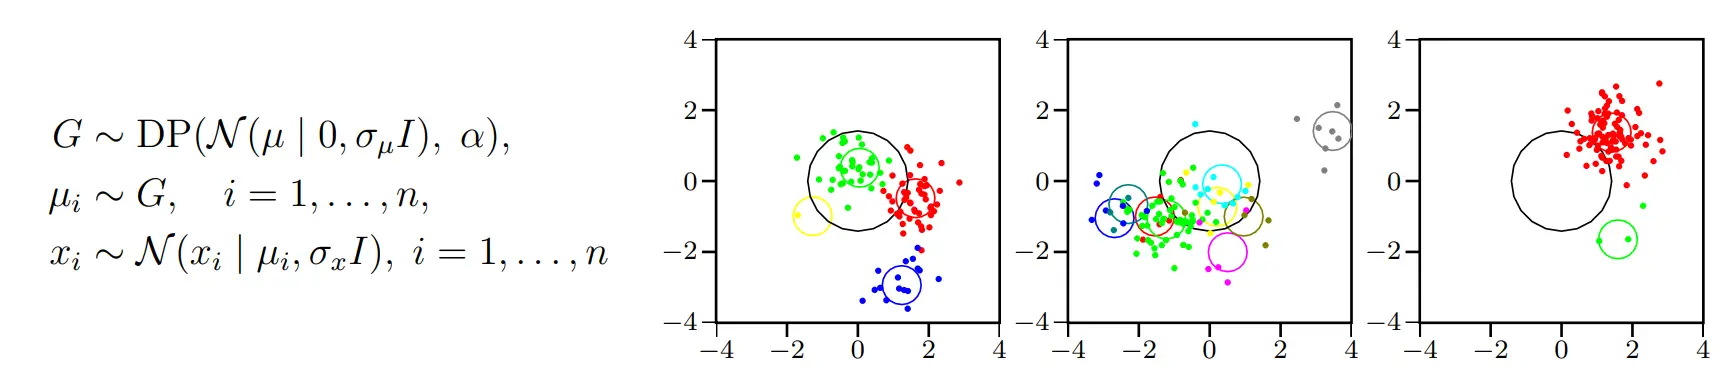
\includegraphics[scale=0.15]{dirichle_sample.png}
		\caption{Примеры генерации выборки}
	\end{center}
	\end{figure}
	\begin{figure}[H]
	\begin{center}
		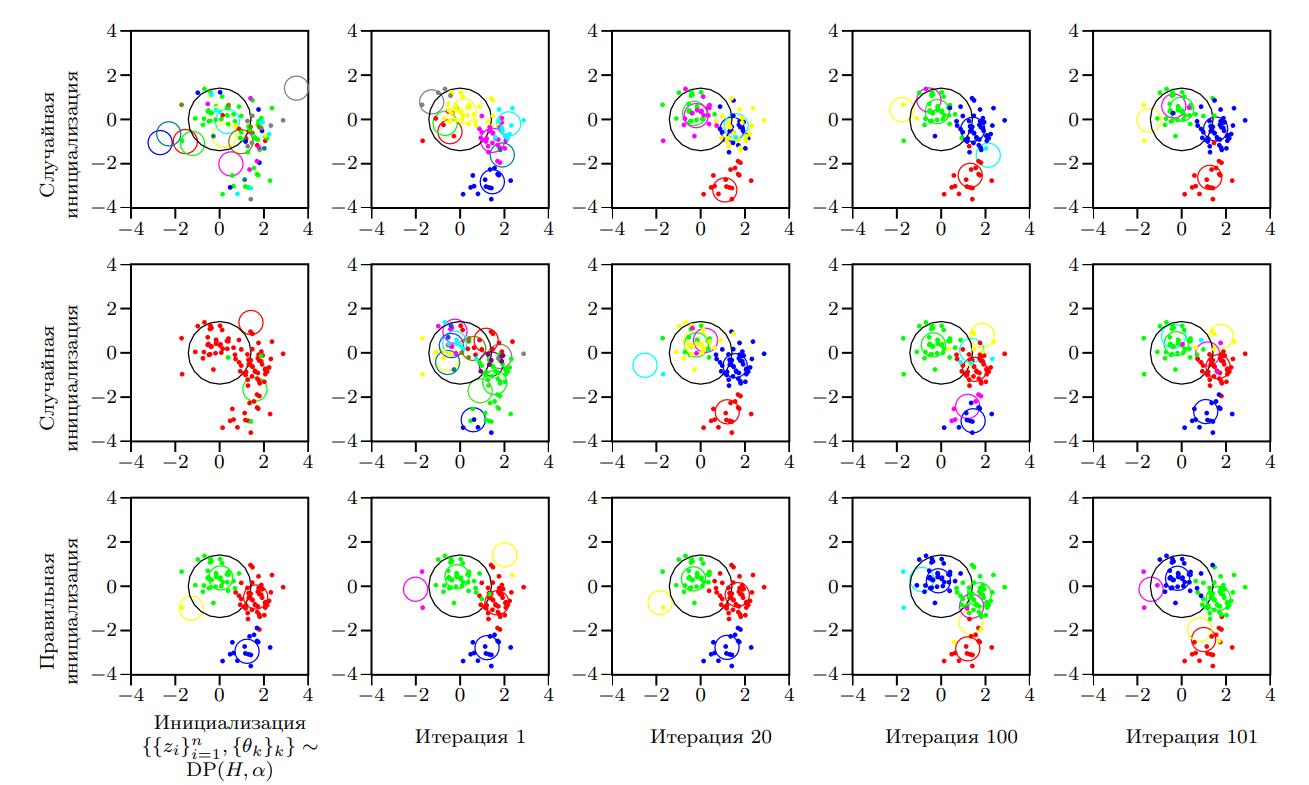
\includegraphics[scale=0.15]{dirichle_result.png}
		\caption{Кластеризация с помощью infinite GMM}
	\end{center}
	\end{figure}
	\end{frame}	
	
	\begin{frame}
	\frametitle{Кластеризация. Спектральная кластеризация}
	Спектральная кластеризация - алгоритм кластеризации, использующий спектр матрицы сходства данных для снижения размерности перед последующей кластеризацией в пространствах меньших размерностей.
	
	Пусть дан граф $G(\mathrm{V}, \mathrm{E})$. Требуется разбить его на 2 непересекающиеся группы ($A, B$) наилучшим в смысле $\phi(A,B)$ образом.
	\vspace{12pt}
	
	$cut(A,B)=\sum\limits_{i \in A, j \in B}w_{ij}$
	\begin{figure}[H]
		\begin{center}
			
\includegraphics[scale=0.1]{graph_cut.png}
		\end{center}
	\end{figure}
	
	$\phi(A,B)=\frac{cut(A,B)}{\min(vol(A), vol(B))} \rightarrow \min$
	\end{frame}	
	
	\begin{frame}
	\frametitle{Кластеризация. Спектральная кластеризация}
	Матрица смежности $\mathrm{A}\ (n\times n)$ для неориентированного графа симметрична, а значит обладает действительными собственными значениями и ортогональным базисом из собственных векторов. Матрица $\mathrm{D}$ -- диагональная матрица, диагональные элементы которой являются степенями соответствующих вершин. Зададим Лапласиан $\mathrm{L}=\mathrm{D}-\mathrm{A}$, все его собственные числа неотрицательны. Тривиальным собственным числом и собственным вектором Лапласиана являются 0 и $\mathbf{1}_n$ соответственно.
	
	Для симметричных матриц верно: 
	$\lambda_2=\min\limits_{x:x^{\mathrm{T}}w_1=0}\frac{x^{\mathrm{T}}\mathrm{M}x}{x^{\mathrm{T}}x}$, тогда
	\begin{equation}
	\label{lambda}
	\lambda_2=\min\limits_{x:\sum{x_i}=0}\sum\limits_{(i,j)\in\mathrm{E}}(x_i-x_j)^2.
	\end{equation}
	\end{frame}
	
	\begin{frame}
	\frametitle{Кластеризация. Спектральная кластеризация}
	$(\ref{lambda}$) минимально, когда $x$ -- собственный вектор (вектор Фидлера), соответствующий $\lambda_2$. Если мы разделим граф по знаку компонент вектора Фидлера, то получим близкое к оптимальному решение в смысле $\phi(A,B)$.
	
	\begin{minipage}{0.45\textwidth}
		\centering
		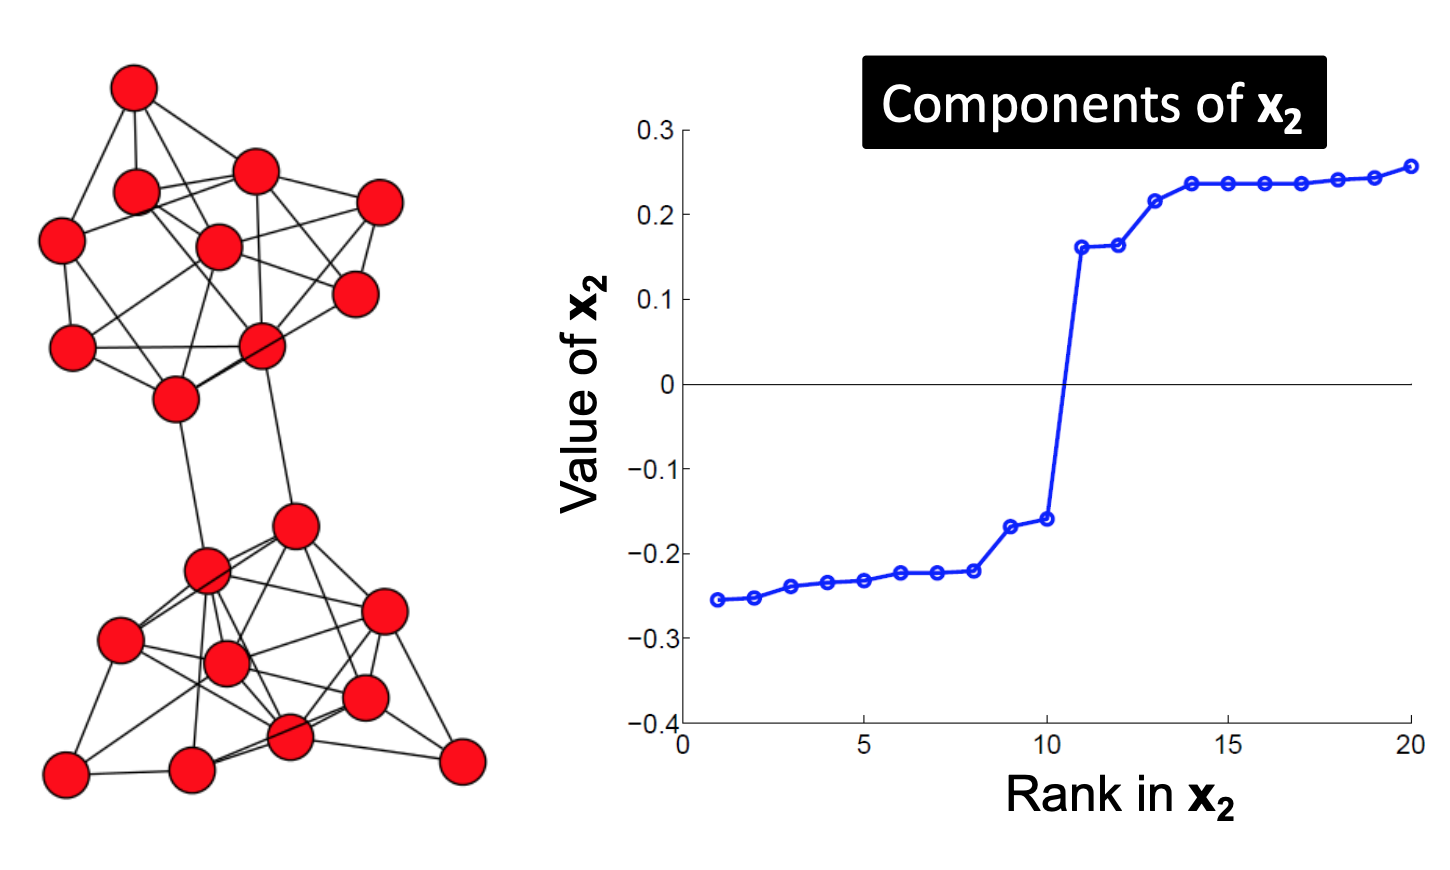
\includegraphics[scale=0.1]{graph_example1.png}
	\end{minipage}\hfill
	\begin{minipage}{0.45\textwidth}
		\centering
		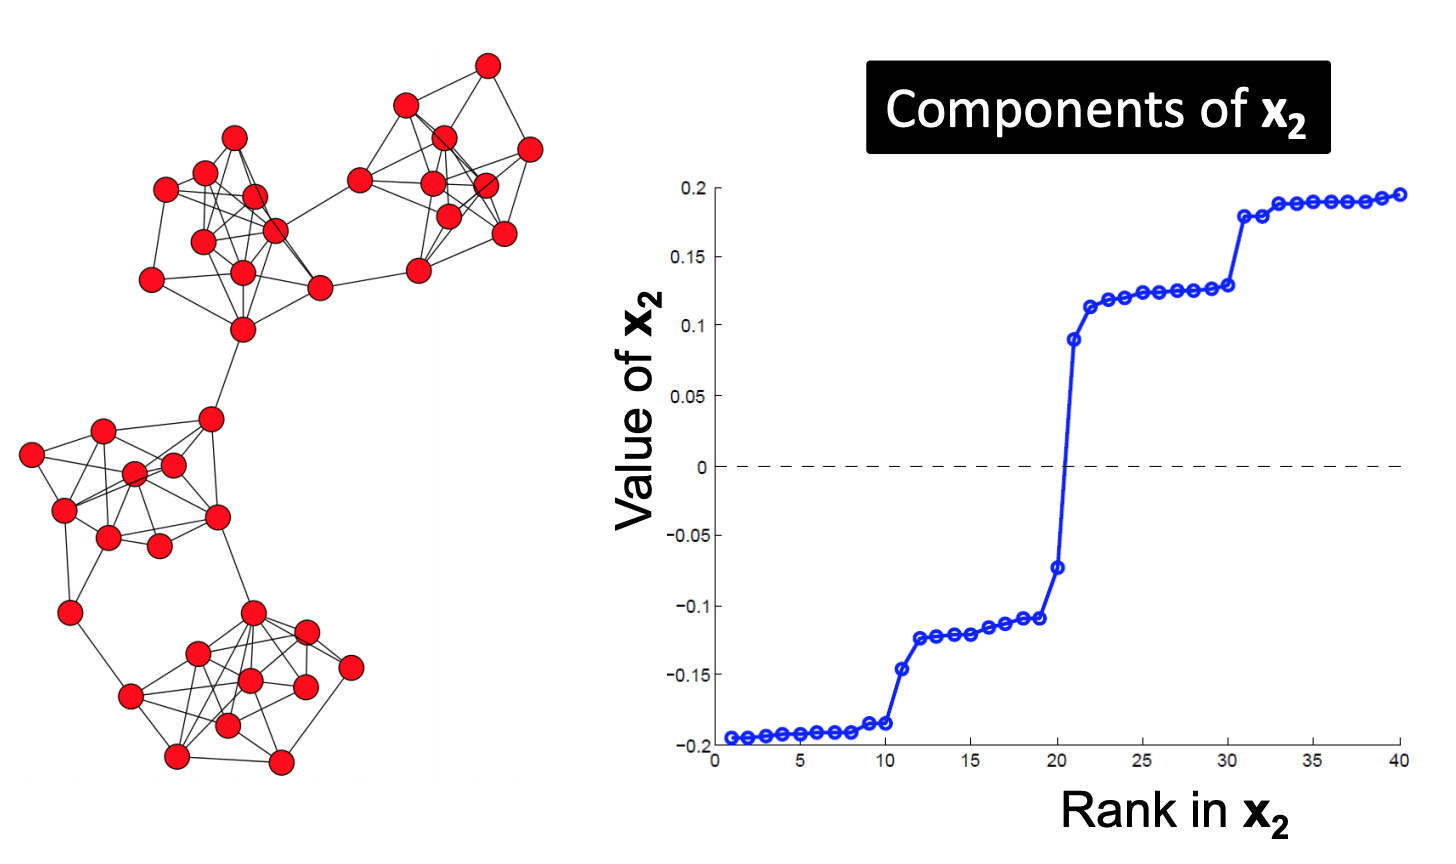
\includegraphics[scale=0.1]{graph_example2.png}
	\end{minipage}
	\begin{figure}[H]
	\begin{center}
		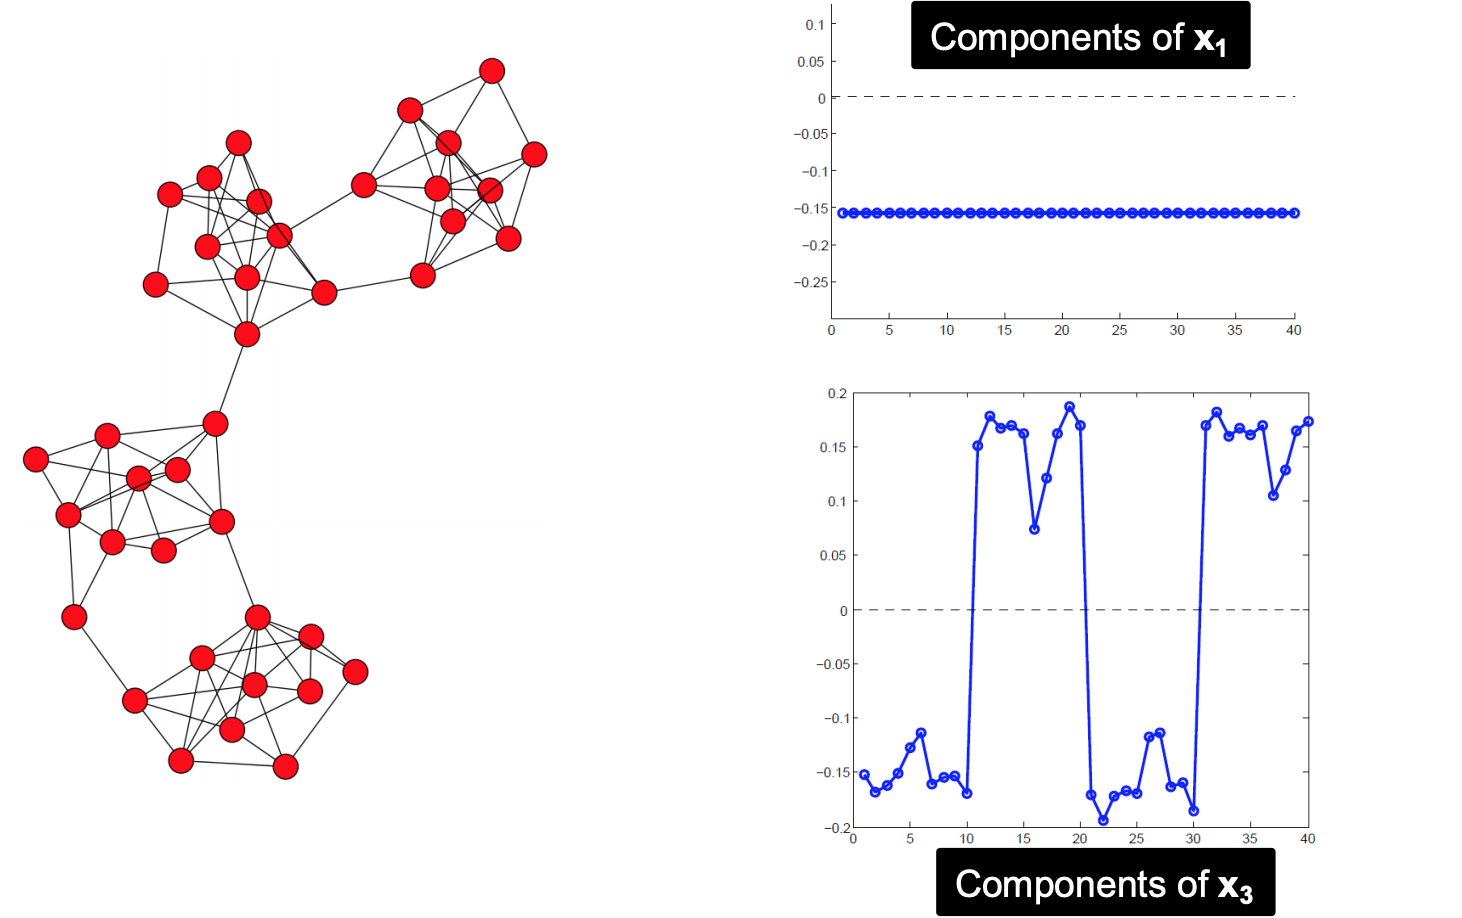
\includegraphics[scale=0.1]{graph_example3.png}
	\end{center}
	\end{figure}
	\end{frame}
	
	\begin{frame}
	\frametitle{Кластеризация. Спектральная кластеризация}
	\textbf{Вход:} выборка $\pmb X^{n} = \{\pmb x_1, \dots, \pmb x_{n}\}$, способ задания матрицы смежности $\mathrm{A}$, количество кластеров $k$, количество собственных векторов $l$, способ кластеризации в пространстве меньшей размерности;

	\textbf{Выход:} разбиение выборки на кластеры;
	\begin{enumerate}
	\item Задаем матрицу $\mathrm{A}$; 
	\item Находим $l$ собственных векторов $\mathrm{L}$ с наименьшими с.ч.; 
	\item \textbf{Если} последовательный метод;
	\item \quad \textbf{Пока} число кластеров < $k$; 
	\item \quad \quad Делим на 2 кластера $A, B$ по знакам элементов $w_2$;
	\item \quad \quad Применяем алгоритм к одному из имеющихся кластеров с $k$, меньшим на 1.
	\item \textbf{Иначе} применяем алгоритм нахождения $k$ кластеров (например, k-means) для матрицы, столбцами которой являются $l$ собственных векторов из шага 2.
	\end{enumerate}
	\end{frame}
	
	\begin{frame}
	\frametitle{Кластеризация. Спектральная кластеризация}
	Способы задания матрицы $\textrm{A}$:
	\begin{enumerate}
	\item RBF: $a_{i,j}=\exp(-\frac{||x_i-x_j||^2}{2\sigma^2})$, $\sigma$ -- параметр
	\item Cosine Similarity: $a_{i,j}=\frac{x_i\cdot x_j}{||x_i||||x_j||}$
	\item Матрица смежности для графа $k$ (или $\varepsilon$) ближайших соседей ($k$ -- не число кластеров, а параметр)
	\end{enumerate}
	Для определения числа кластеров можно использовать метод локтя для собственных чисел. Вместо $\mathrm{L}$ можно использовать нормированные версии:
	$\mathrm{L_{sym}}=\mathrm{E}-\mathrm{D}^{-1/2}\mathrm{A}\mathrm{D}^{-1/2}$,
	$\mathrm{L_{rw}}=\mathrm{E}-\mathrm{D}^{-1}\mathrm{A}$.
	
	\textbf{Достоинства}: Хорошо работает для кластеров сложной формы, понижает размерность данных, много гиперпараметров.
	
	\textbf{Недостатки}: Высокая вычислительная сложность и потребление памяти, чувствителен к выбросам, шуму и выбору гиперпараметров. 
	\end{frame}
	
	\begin{frame}
	\frametitle{Кластеризация. Алгоритм DBSCAN}
	\textbf{DBSCAN} (Density-based spatial clustering of applications with noise) --- это эвристический алгоритм кластеризации, который предложили Маритин Эстер, Ганс-Петер Кригель, Ёрг Сандер и Сяовэй Су в 1996. Это алгоритм кластеризации, основанный на плотности --- алгоритм группирует вместе те объекты, которые тесно расположены, помечая как выбросы объекты, которые находятся в областях с малой плотностью.

	
В этом алгоритме рассматривается для каждого объекта $\pmb x \in U$ его $\varepsilon$-окрестность $U_\varepsilon (\pmb x) = \{\pmb u \in U : \rho(\pmb x , \pmb u ) \leq \varepsilon\}$.
	\end{frame}
	
	\begin{frame}
	\frametitle{Кластеризация. Алгоритм DBSCAN}
	В этом алгоритме рассматривается для каждого объекта $\pmb x \in U$ его $\varepsilon$-окрестность $U_\varepsilon (\pmb x) = \{\pmb u \in U : \rho(\pmb x , \pmb u ) \leq \varepsilon\}$.
	
Каждый объект может быть одного из трёх типов:
	\begin{itemize}
		\item корневой: имеет плотную окрестность $|U_\varepsilon (\pmb x)| \geq m$ 
		\item граничный: не корневой, но находится в окрестности корневого 
		\item выброс: не корневой и не граничный. 
	\end{itemize}
	\end{frame}
	
	\begin{frame}
	\frametitle{Кластеризация. Алгоритм DBSCAN}
	
	\begin{figure}[H]
		\begin{center}
			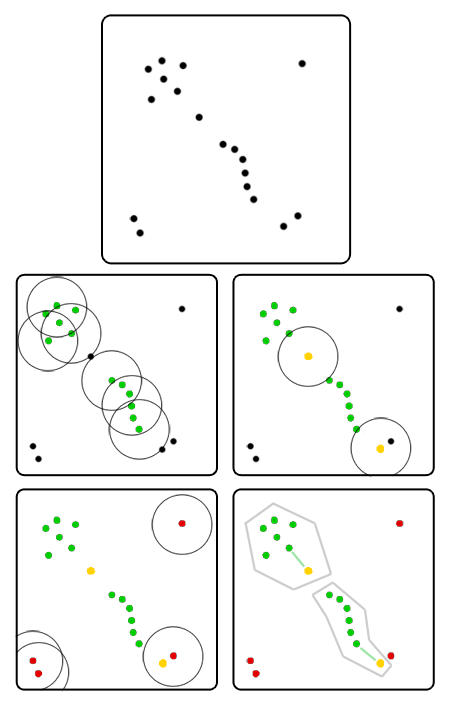
\includegraphics[scale = 1.1]{dbscan.png}
			\caption{Иллюстрация к алгоритму DBSCAN. На рисунке зелёным отмечены корневые объекты, жёлтым~---~граничные и красным~---~шумовые.}
		\end{center}
	\end{figure}
	Корневые объекты находящиеся в $\varepsilon$-окрестности друг друга объединяются в один кластер. Граничные объекты относятся к тому кластеру, к какому относится корневой
	объект, в $\varepsilon$-окрестности которого лежит данный граничный объект. Таким образом, в итоге получается разделение всех объектов на кластеры и шумовые объекты.

	\end{frame}
	
	\begin{frame}
	\frametitle{Кластеризация. Алгоритм DBSCAN}
	

	Корневые объекты находящиеся в $\varepsilon$-окрестности друг друга объединяются в один кластер. Граничные объекты относятся к тому кластеру, к какому относится корневой
	объект, в $\varepsilon$-окрестности которого лежит данный граничный объект. Таким образом, в итоге получается разделение всех объектов на кластеры и шумовые объекты.

	\end{frame}
	
	\begin{frame}
	\frametitle{Кластеризация. Алгоритм DBSCAN}
	

	\textbf{Вход:} выборка $\pmb X^{n} = \{\pmb x_1, \dots, \pmb x_{n}\}$, параметры $\varepsilon$ и $m$;
	
\textbf{Выход:} разбиение выборки на кластеры и шумовые выбросы;
\begin{enumerate}
		\item $U=X^n$, $a=0$; 
		\item \textbf{Пока} есть некластеризованные точки, т.е. $U \neq \varnothing$; 
		\item \quad взять случайную точку $\pmb x \in U$; 
		\item \quad \textbf{если} $|U_\varepsilon (\pmb x)| < m$, \textbf{то} 
		\item \quad \quad пометить $\pmb x$ как шумовой; 
		\item \quad \textbf{иначе} 
		\item \quad \quad создать новый кластер: $K=U_\varepsilon (\pmb x)$; $a = a + 1$; 
		\item \quad \quad \textbf{для всех} $\pmb x' \in K$ 
		\item \quad \quad \quad \textbf{если} $|U_\varepsilon (\pmb x')| \geq m$ \textbf{то} $K=K \cup U_\varepsilon(\pmb x')$; 
		\item \quad \quad \quad \textbf{иначе} пометить $\pmb x'$ как граничный элемент $K$; 
		\item \quad \quad соотнести объект классу $a$ для всех $\pmb x' \in K$; 
		\item \quad \quad $U=U \setminus K$ 
\end{enumerate}

	\end{frame}
	
	\begin{frame}
	\frametitle{Кластеризация. Алгоритм DBSCAN}
	

	\textbf{Достоинства:} 
\begin{itemize}
	\item Относительно быстрая кластеризация больших данных (от $O(n \ln n)$ до $O(n^2)$ в зависимости от реализации); 
	\item Позволяет обрабатыват кластеры произвольной формы (в том числе протяжённые ленты, концентрические гиперсферы); 
	\item Помимо деления на кластеры выдаёт ещё и разметку шумовых объектов; 
	\item Cам определяет количество кластеров (по модулю задания других гиперпараметров);
	\item Хорошо поддаётся модифицированию (существуют реализации, скрещенные с k-means, например). 
\end{itemize}

\textbf{Недостатки:}\\ 
	Алгоритм может неадекватно обрабатывать сильные вариации плотности данных внутри кластера, проёмы и шумовые мосты между кластерами.
	То есть метод не способен соединять кластеры через проёмы, и, наоборот, связывает явно различные кластеры через плотно населённые перемычки. Проблема особенно актуальна для данных большой размерности, так как чем больше $p$, тем больше мест, где могут случайно возникнуть проёмы или мосты.

	\end{frame}
	
	\begin{frame}
	\frametitle{Кластеризация. Оценка результата}
	

	\textbf{Среднее внутрикластерное расстояние} 
$$F_0 = \frac{\sum_{i < j}\mathbf{I}_{\{y_i = y_j\}}\rho(\pmb x_i, \pmb x_j)}{\sum_{i < j}\mathbf{I}_{\{y_i = y_j\}}},$$ 

Решая задачу кластеризации, мы хотим по возможности получать как можно более кучные кластеры, то есть минимизировать $F_0$.

	\textbf{Среднее межкластерное расстояние} 
	$$F_1 = \frac{\sum_{i < j}\mathbf{I}_{\{y_i \neq y_j\}}\rho(\pmb x_i, \pmb x_j)}{\sum_{i < j}\mathbf{I}_{\{y_i \neq y_j\}}}.$$

Среднее межкластерное расстояние, напротив, нужно максимизировать, то есть целесообразно выделять в разные кластеры наиболее удалённые друг от друга объекты.

Имеет смысл вычислять отношение пары функционалов, чтобы учесть как внутрикластерные, так и межкластерные расстояния: $F_0/F_1 \rightarrow min$.

	\end{frame}
	
	\begin{frame}
	\frametitle{Кластеризация. Оценка результата}
	\textbf{Коэффициент силуэта} 
	$$s(i) = \frac{b(i) - a(i)}{\max(a(i), b(i))}.$$
	$$\text{DBI} = \frac{1}{k} \sum_{i=1}^{k} \max_{i \neq j} \left( \frac{s_i + s_j}{d_{ij}} \right).$$
	\end{frame}
	
		\begin{frame}
	\frametitle{Кластеризация}
	\begin{figure}[H]
	\begin{center}
		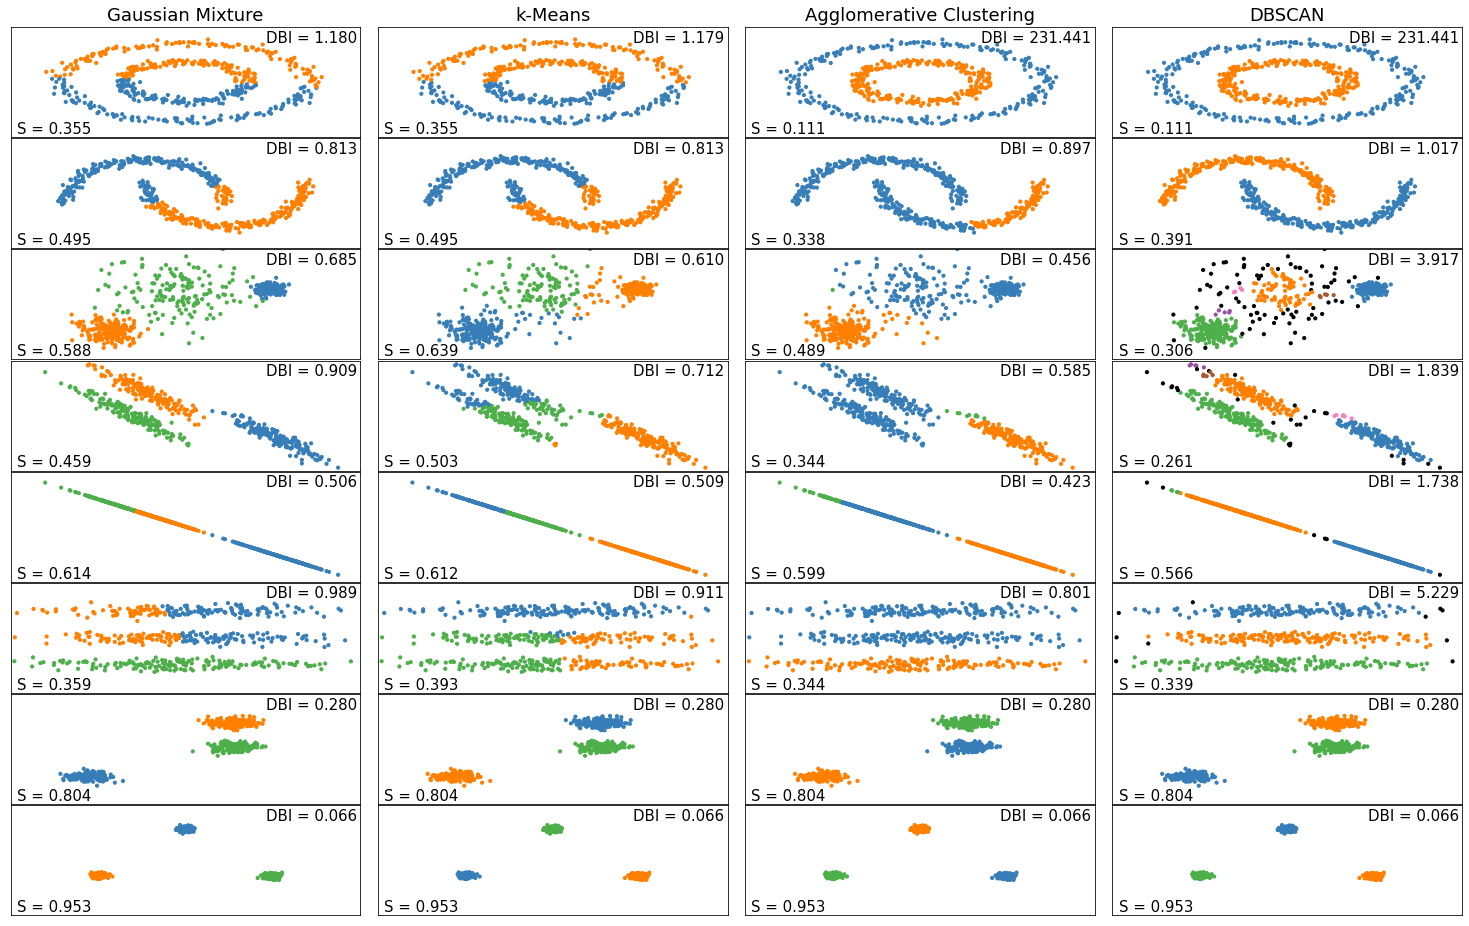
\includegraphics[scale = 0.2]{qual.png}
		\caption{Сравнение результатов работы различных алгоритмов кластеризации}
	\end{center}
\end{figure}

	\end{frame}
	
	\begin{frame}
	\frametitle{Тематическое обучение. Введение}
	Тематическое моделирование --- технология статистического анализа текстов для автоматического выявления тематики в больших коллекциях документов.
	
	Чем-то похоже на кластеризацию, но тематическое моделирование в этом плане является «мягким» и допускает, чтобы документ относился к нескольким кластерам-темам. Тематическое моделирование не претендует на понимание смысла текста, однако оно способно отвечать на вопросы «о чём этот текст» или «какие общие темы имеет эта пара текстов».
	\end{frame}
	
	\begin{frame}
	\frametitle{Тематическое обучение. Параметры тематической модели }
	

	\begin{itemize}
	\item $p(\omega | t)$  --- матрица искомых условных распределений слов по темам;
	\item $p(t | d)$ --- матрица искомых условных распределений тем по документам;
	\item $d$ --- документ;
	\item $\omega$ --- слово;
	\item $d,\omega$  --- наблюдаемые переменные;
	\item $t$  --- тема (скрытая переменная).
\end{itemize}


	\end{frame}
	
	\begin{frame}
	\frametitle{Тематическое обучение. Параметры тематической модели }
	

\begin{figure}[H]
	\begin{center}
		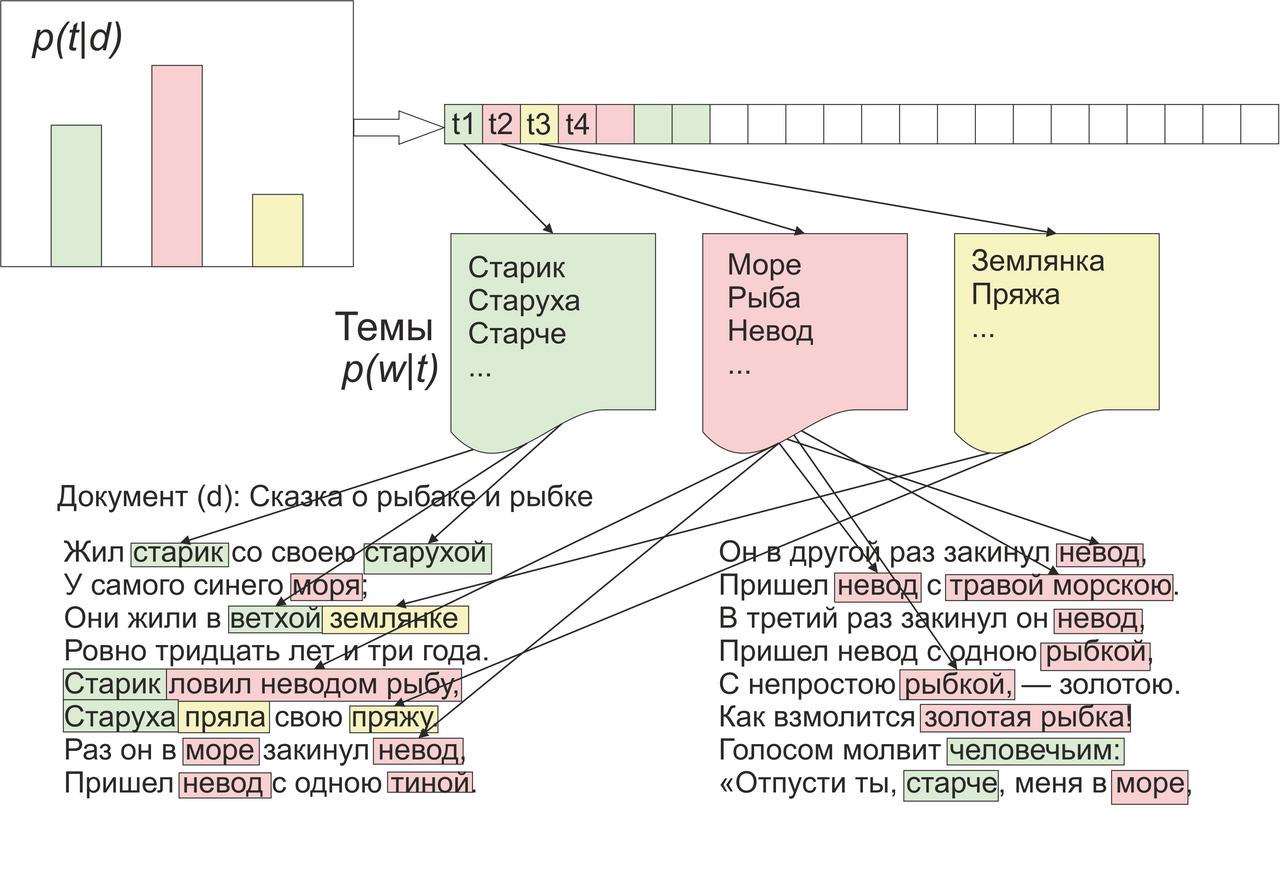
\includegraphics[scale = 1]{TM.png}
		\caption{Иллюстрация параметров модели тематического обучения.}
	\end{center}
\end{figure}
	\end{frame}
	
	\begin{frame}
	\frametitle{Тематическое обучение. LSA}
	
Латентно-семантический анализ, LSA (latent semantic analysis), он же LSI (latent semantic indexing) --- самая ранняя модель, предложенная еще в конце 80-х гг. Модель называется латентной, т.к. предполагает введение скрытого (латентного) параметра — темы.

LSA основан на использовании сингулярного разложения матрицы. С помощью SVD-разложения любая матрица раскладывается во множество ортогональных матриц, линейная комбинация которых является достаточно точным приближением к исходной матрице. Этим и объясняется название этого алгоритма в sklearn — TruncaredSVD.


	\end{frame}
	
		\begin{frame}
	\frametitle{Тематическое обучение. LSA}
	

\begin{figure}[H]
	\begin{center}
		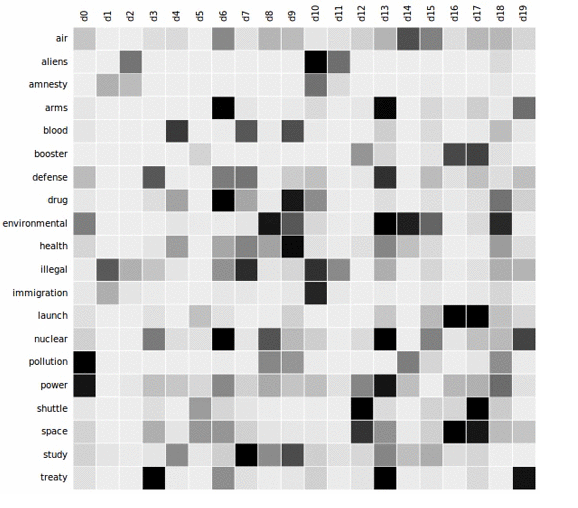
\includegraphics[scale = 0.4]{LSA1.png}
		\caption{Иллюстрация SVD в методе LSA (исходная матрица).}
	\end{center}
\end{figure}

	\end{frame}
	
			\begin{frame}
	\frametitle{Тематическое обучение. LSA}
	

\begin{figure}[H]
	\begin{center}
		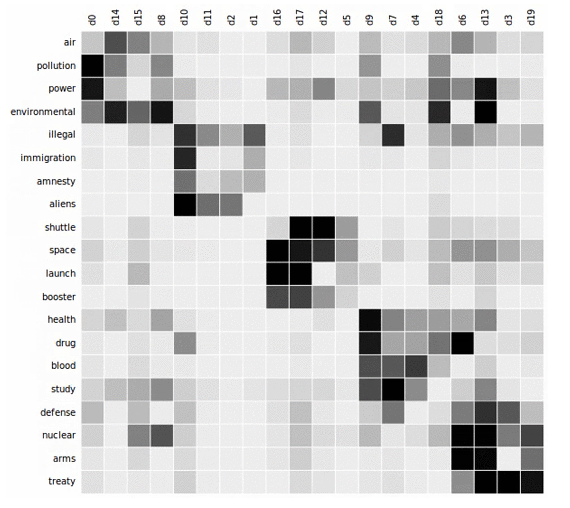
\includegraphics[scale = 0.4]{LSA2.png}
		\caption{Иллюстрация SVD в методе LSA.}
	\end{center}
\end{figure}

	\end{frame}
		\begin{frame}
	\frametitle{Тематическое обучение. pLSA}
	

pLSA (probabilistic latent semantic analysis), она же pLSI (probabilistic latent semantic indexing) --- вероятностный латентно-семантический анализ (индексирование). Модель предложена в 1999 г. Томасом Хоффманом.

Зачем понадобилось модифицировать LSA? Проблема этого метода в том, что он предполагает, что слова и документы имеют нормальное распределение, но в реальности это не так. Поэтому на практике чаще используется pLSA, основанный на мультиномиальном распределении. Если LSA — это чистая линейная алгебра, то pLSA имеет еще и статистические основания.

	\end{frame}
	
			\begin{frame}
	\frametitle{Тематическое обучение. pLSA}
	

\textbf{Дана} коллекция текстовых документов (мешок слов): $n_{d\omega}$ --- сколько раз термин $\omega$ встречаетсяя в документе $d$.

\textbf{Найти} модель $p(\omega | d) = \sum_t \phi_{\omega t}\theta_{td}$ с параметрами $\phi, \theta$:

\begin{itemize}
	\item $\phi_{\omega t} = p(\omega | t)$  --- вероятности терминов $\omega$ в каждой теме $t$;
	\item $\theta_{td} = p(t | d)$ --- вероятности тем $t$ в каждом документе $d$.
\end{itemize}

	\end{frame}
	
	\begin{frame}
	\frametitle{Тематическое обучение. pLSA}
	

Неизвестная модель находится путем максимизации логарифма правдоподобия:

$$ \sum_{d,\omega} n_{d,\omega} ln \sum_{t} \phi_{\omega t}\theta_{td} \rightarrow  \max_{\phi, \theta}$$

при ограничениях нормировки и неотрицательности:

$$ \phi_{\omega t} \geq 0; \sum_{\omega} \phi_{\omega t} = 1; \theta_{td} \geq 0; \sum_{t} \theta_{td} = 1$$

	\end{frame}
	
		\begin{frame}
	\frametitle{Тематическое обучение. pLSA}
	
Точка максимума правдоподобия $\phi, \theta$ удовлетворяет системе уравнений со вспомогательными переменными $p_{td\omega}$:
$$
\begin{cases}
\displaystyle
p_{td\omega}={ {\phi_{\omega t} \theta_{td} } \over { \sum_{t'} \phi_{\omega t'} \theta_{t'd}}}\\
\phi_{\omega t} = { {n_{\omega t}} \over {\sum_{\omega `} n_{\omega `t}}}; n_{\omega t} = \sum_{d \in D} n_{d\omega}p_{td\omega}\\
\theta_{td} = { {n_{td}} \over {\sum_{t'}n_{t'd}}}; n_{td} = \sum_{\omega \in d} n_{d\omega}p_{td\omega}
\end{cases}
$$

Где первое уравнение это $E$-шаг $EM$ алгоритма, а второе и третье уравнение --- $M$-шаг.

	\end{frame}
	
			\begin{frame}
	\frametitle{Тематическое обучение. pLSA}
	
\textbf{$E$-шаг -- это формула Байеса:}

$$p_{td\omega} = p(t | d, \omega) = { {p(\omega , t | d)} \over {p(\omega | d)}} = { {p(\omega | t) p(t|d)} \over {p(\omega | d)}}= {{\phi_{\omega t}\theta_{td}} \over {\sum_{s \in T}\phi_{\omega t}\theta_{td}}}$$

$n_{d \omega t} = n_{d \omega}p(t | d, \omega)$ --- оценка числа троек $(d, \omega, t)$ в коллекции
	\end{frame}

		\begin{frame}
	\frametitle{Тематическое обучение. pLSA}
	
\textbf{$M$-шаг --- это частотные оценки условных вероятностей:}

$$ \phi_{\omega t} = {{n_{\omega t}} \over {n_t}} \equiv {{\sum_{d \in D} n_{d \omega t}} \over {\sum_{d \in D} \sum_{\omega \in d} n_{d \omega t}}} $$

$$ \theta_{td} = { {n_td} \over {n_d}} \equiv {{\sum_{\omega \in D} n_{d \omega t}} \over {\sum_{\omega \in \Omega} \sum_{t \in T} n_{d \omega t}}}$$
	\end{frame}
	
			\begin{frame}
	\frametitle{Тематическое обучение. pLSA}
	
\textbf{Вход:} коллекция $D$, число тем $|T|$ и число иттераций $i_{max}$;
	
\textbf{Выход:} матрица терминов тем $\Theta$ и тем документов $\Phi$;

\begin{enumerate}
		\item инициализация $\phi_{\omega t}, \theta_{td}$ для всех $d \in D, \omega \in \Omega, t \in T$; 
		\item \textbf{для всех} иттераций $i=1, \cdots, i_{max}$ 
		\item \quad $n_{\omega t}, n_{td}, n_t, n_d := 0$ для всех $d \in D, \omega \in \Omega, t \in T$; 
		\item \quad \textbf{для всех} документов  $d \in D$ и слов $\omega \in d$
		\item \quad \quad $p_{td\omega} = {{\phi_{\omega t} \theta_{td}} \over {\sum_{s} \phi_{\omega s} \theta_{sd}}}$; 
		\item \quad \quad $n_{\omega t}, n_{td}, n_t, n_d += n_{d \omega} p_{td \omega}$ для всех $t \in T$;
		\item \quad $\phi_{\omega t} := n_{\omega t}/n_t$ для всех $\omega \in \Omega, t \in T$;
		\item \quad $\phi_{td} := n_{td}/n_d$ для всех $d \in D, t \in T$;

\end{enumerate}
	\end{frame}
\end{document}